\documentclass[answers]{exam}
\usepackage[english]{babel}
\usepackage[utf8x]{inputenc}
\usepackage{amsmath,amssymb,amsthm}

\title{OPER 510 - Introduction to Mathematical Programming%
	\\ Assignment 6}
\author{Brandon Hosley}
\date{\today}

\usepackage[table,dvipsnames,xcdraw]{xcolor}
\usepackage{graphicx}
\usepackage{enumitem}

\usepackage{booktabs}

\usepackage{tabularx,makecell,diagbox}
\newcolumntype{Y}{>{\centering\arraybackslash}X}

\usepackage{pgf,tikz,tikz-3dplot}
\usetikzlibrary{shapes,arrows,positioning,backgrounds}
\tikzset{%
roundnode/.style={circle, draw=MidnightBlue!90, thick, fill=gray!40},
pt/.style={draw=MidnightBlue, thick,->,>=stealth',shorten >=1pt},
bid/.style={draw=MidnightBlue, thick,-}
}



\usepackage{float}

\begin{document}
\maketitle
\unframedsolutions

\begin{questions}
% Problem 1
\question \textit{Page 398, Problem 1 in Winston} \\
Five employees are available to perform four jobs. The time it takes each person to perform each job is given in Table 50. Determine the assignment of employees to jobs that minimizes the total time required to perform the four jobs.
\begin{center}
	\setlength{\aboverulesep}{0pt}
	\setlength{\belowrulesep}{0pt}
	\setlength{\extrarowheight}{.75ex}
	\arrayrulecolor{Blue}
	\begin{tabular}{lcccc}
		\toprule
		\rowcolor{gray!25}
		& \multicolumn{4}{c}{  \textbf{\textcolor{Blue}{Time (hours)}}  }  \\ 
		\cline{2-5} \rowcolor{gray!25}
		\textbf{\textcolor{Blue}{Person}} & \textbf{\textcolor{Blue}{Job 1}} & \textbf{\textcolor{Blue}{Job 2}} & \textbf{\textcolor{Blue}{Job 3}} & \textbf{\textcolor{Blue}{Job 4}}  \\
		\midrule
		1 & 22 & 18 & 30 & 18 \\
		2 & 18 & —  & 27 & 22 \\
		3 & 26 & 20 & 28 & 28 \\
		4 & 16 & 22 &  — & 14 \\
		5 & 21 & —  & 25 & 28 \\
		\bottomrule[2pt]
	\end{tabular}
	%\caption{\textit{Note:} Dashes indicate person cannot do that particular job.}
\end{center}

\begin{solution}
\end{solution}


% Problem 2
\question \textit{Page 459, Problem 2 in Winston} \\
The city of Smalltown consists of five subdivisions. Mayor John Lion wants to build telephone lines to ensure that all the subdivisions can communicate with each other. The distances between the subdivisions are given in Figure 50. What is the minimum length of telephone line required? Assume that no telephone line can be built between subdivisions 1 and 4.

\begin{figure}[H]
	\centering
	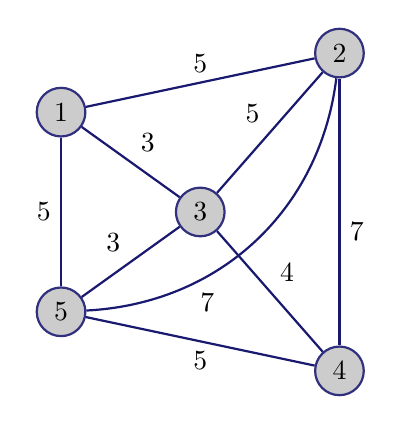
\begin{tikzpicture}[node distance=2.5cm]
		\node[roundnode] (three) [] {3};
		\node[roundnode] (one) [above left of=three, yshift=-0.5cm] {1};
		\node[roundnode] (two) [above right of=three, yshift=0.25cm] {2};
		\node[roundnode] (four) [below right of=three, yshift=-0.25cm] {4};
		\node[roundnode] (five) [below left of=three, yshift=0.5cm] {5};
		
		\path[bid] (one) edge [] node [above] {5} (two);
		\path[bid] (one) edge [] node [above right] {3} (three);
		\path[bid] (one) edge [] node [left] {5} (five);
		
		\path[bid] (two) edge [] node [above left] {5} (three);
		\path[bid] (two) edge [] node [below right] {7} (four);
		\path[bid] (two) edge [bend left=40] node [below left, yshift=-15pt, xshift=-11pt] {7} (five);
		
		\path[bid] (three) edge [] node [above right] {4} (four);
		\path[bid] (three) edge [] node [above left] {3} (five);
		
		\path[bid] (four) edge [] node [below] {5} (five);
	\end{tikzpicture}
	\caption[50]{}
\end{figure}

\begin{solution}	
\end{solution}


% Problem 3
\question
You are building a shift schedule for the Air Operations Center with required airmen by four- hour periods given in the table.
\begin{center}
	\begin{tabular}{|l|c|}
		\toprule
		\hspace{13ex} \textbf{Time Period} \hspace{13ex} & \textbf{Required Workers} \\
		\midrule
		2400-0400 hours (Midnight – 4 a.m.) & 4  \\ 
		0400-0800 hours (4 a.m. – 8 a.m.)   & 8  \\
		0800-1200 hours (8 a.m. – Noon)     & 10 \\
		1200-1600 hours (Noon – 4 p.m.)     & 7  \\
		1600-2000 hours (4 p.m. – 8 p.m.)   & 12 \\
		2000-2400 hours (8 p.m. – Midnight) & 4  \\
		\bottomrule
	\end{tabular}
\end{center}

\begin{parts}
	\part Formulate the mathematical program given that the airmen must work consecutive eight- hour shifts that will minimize the total airman required.
	
	\part Solve the model formulated in a) You may use a computer program if you wish. If you do, identify the program used and the number of iterations taken. Be sure to clearly express your solution for transmittal to the Sergeant of the Guard so they can have the proper number of airman available.
\end{parts}

\begin{solution}
\end{solution}


% Problem 4
\question
Solve the shortest path problem for the networks below using Dijkstra’s algorithm. Show all steps.
\begin{figure}[H]
	\centering
	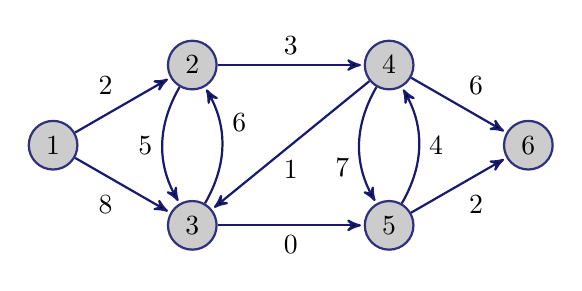
\begin{tikzpicture}[node distance=2.5cm]
		\node[roundnode] (one) {1};
		\node[roundnode] (two) [above right of=one, yshift=-0.75cm] {2};
		\node[roundnode] (three) [below right of=one, yshift=0.75cm] {3};
		\node[roundnode] (four) [right of=two] {4};
		\node[roundnode] (five) [right of=three] {5};
		\node[roundnode] (six) [above right of=five, yshift=-0.75cm] {6};
	
		\path[pt] (one) edge [] node [above left] {2} (two);
		\path[pt] (one) edge [] node [below left] {8} (three);
		
		\path[pt] (two) edge [bend right] node [left] {5} (three);
		\path[pt] (three) edge [bend right] node [right, yshift=8pt] {6} (two);
		
		\path[pt] (two) edge [] node [above] {3} (four);
		\path[pt] (three) edge [] node [below] {0} (five);
		
		\path[pt] (four) edge [bend right] node [left, yshift=-8pt] {7} (five);
		\path[pt] (five) edge [bend right] node [right] {4} (four);
		
		\path[pt] (four) edge [] node [above right] {6} (six);
		\path[pt] (four) edge [] node [below, yshift=-2pt] {1} (three);
		\path[pt] (five) edge [] node [below right] {2} (six);
	\end{tikzpicture}
	% \caption{}
\end{figure}

As Dijkstra’s algorithm is a dynamic program, identify the stages, states and recursive relation used in the approach.

\begin{solution}
\end{solution}


\end{questions}
\end{document}